%Copyright (C) 2014 Sergio García Villalonga.

Per tal de poder dur a terme una avaluació de la influència de la presència d'usuaris en la precisió del sistema de localització en interiors es necessita un lloc que presentàs fortes diferències en el nombre de persones presents a l'entorn. A més, tenint en compte que el sistema AirPlace es basa en la localització mitjançant una infraestructura WiFi existent, l'entorn ha de proveir una quantitat suficient de punts d'accés per dur a terme les nostres operacions.

Aquestes necessitats es veuen cobertes en edificis com els centres comercials. Les proves realitzades per aquest estudi es varen dur a terme en una secció del centre comercial Glòries, a Barcelona. La diferència horària entre l'obertura del centre als treballadors i l'obertura als clients proporciona un context idoni per realitzar proves en un entorn pràcticament buit als matins, i la proximitat de les festes de Nadal a la hora de realitzar les proves han ofert un entorn molt concorregut durant l'horari comercial.

A més, l'elecció d'un centre comercial, proporciona dos tipus d'espais -passadissos i botigues- sobre els que resulta interessant classificar els resultats, ja que presenten característiques que afecten a la precisió.
En el cas dels passadissos, l'entorn es caracteritza per:

\begin{itemize}
    \item Majors espais.
    \item Voltes més amples.
    \item Menys presència d'obstacles entre diferents punts.
\end{itemize}

Per contra, les botigues proporcionen un context en el que, a priori, la precisió es pot veure minvada, tant en el cas d'absència com en el de presència d'usuaris en l'entorn degut, entre d'altres a:

\begin{itemize}
    \item Presència de prestatges.
    \item Parets més properes.
    \item Mostres més baixos.
\end{itemize}

La realització de les proves dins un centre comercial i l'estudi els resultats dels dos tipus de localitzacions pot permetre, a més d'afrontar possibles millores de la manera més adequada en cada situació, donar un enfocament a una situació més realista que no al realitzar proves planificades dins un entorn controlat com pot ser un laboratori.

El primer pas és la creació del mapa de ràdio, que consisteix en recaptar, en diferents localitzacions, informació sobre quins punts d'accés WiFi es localitzen i amb quina intensitat es capta el senyal. Amb aquesta informació, a la hora d'estimar una posició a posteriori, s'apliquen diferents algorismes que contrasten la informació del mapa de ràdio amb la informació sobre punts d'accés i intensitats que detecta l'usuari del sistema.

\subsection{Creació del mapa de ràdio}

A la hora de crear el mapa de ràdio s'han tingut en compte una sèrie de consideracions. La primera és on prendre les mesures per realitzar les mesures. En l'estudi, s'ha intentat realitzar una presa de dades amb punts distribuïts més o menys uniformement per tot l'edifici. La impossibilitat d'obtenir plànols detallats de l'interior de les botigues i el fet de que alguns locals es troben tancats, ha afectat a la uniformitat d'aquesta distribució, situació que no es dóna en les mostres preses als passadissos.

En la figura \ref{fig:planol_log} es pot veure els punts que representen la presa de dades del mapa de ràdio sobre el plànol. En total s'han pres 83 mostres, amb una distància mínima mitjana entre punts de 8,23 m.

\begin{figure}[ht]
\begin{center}
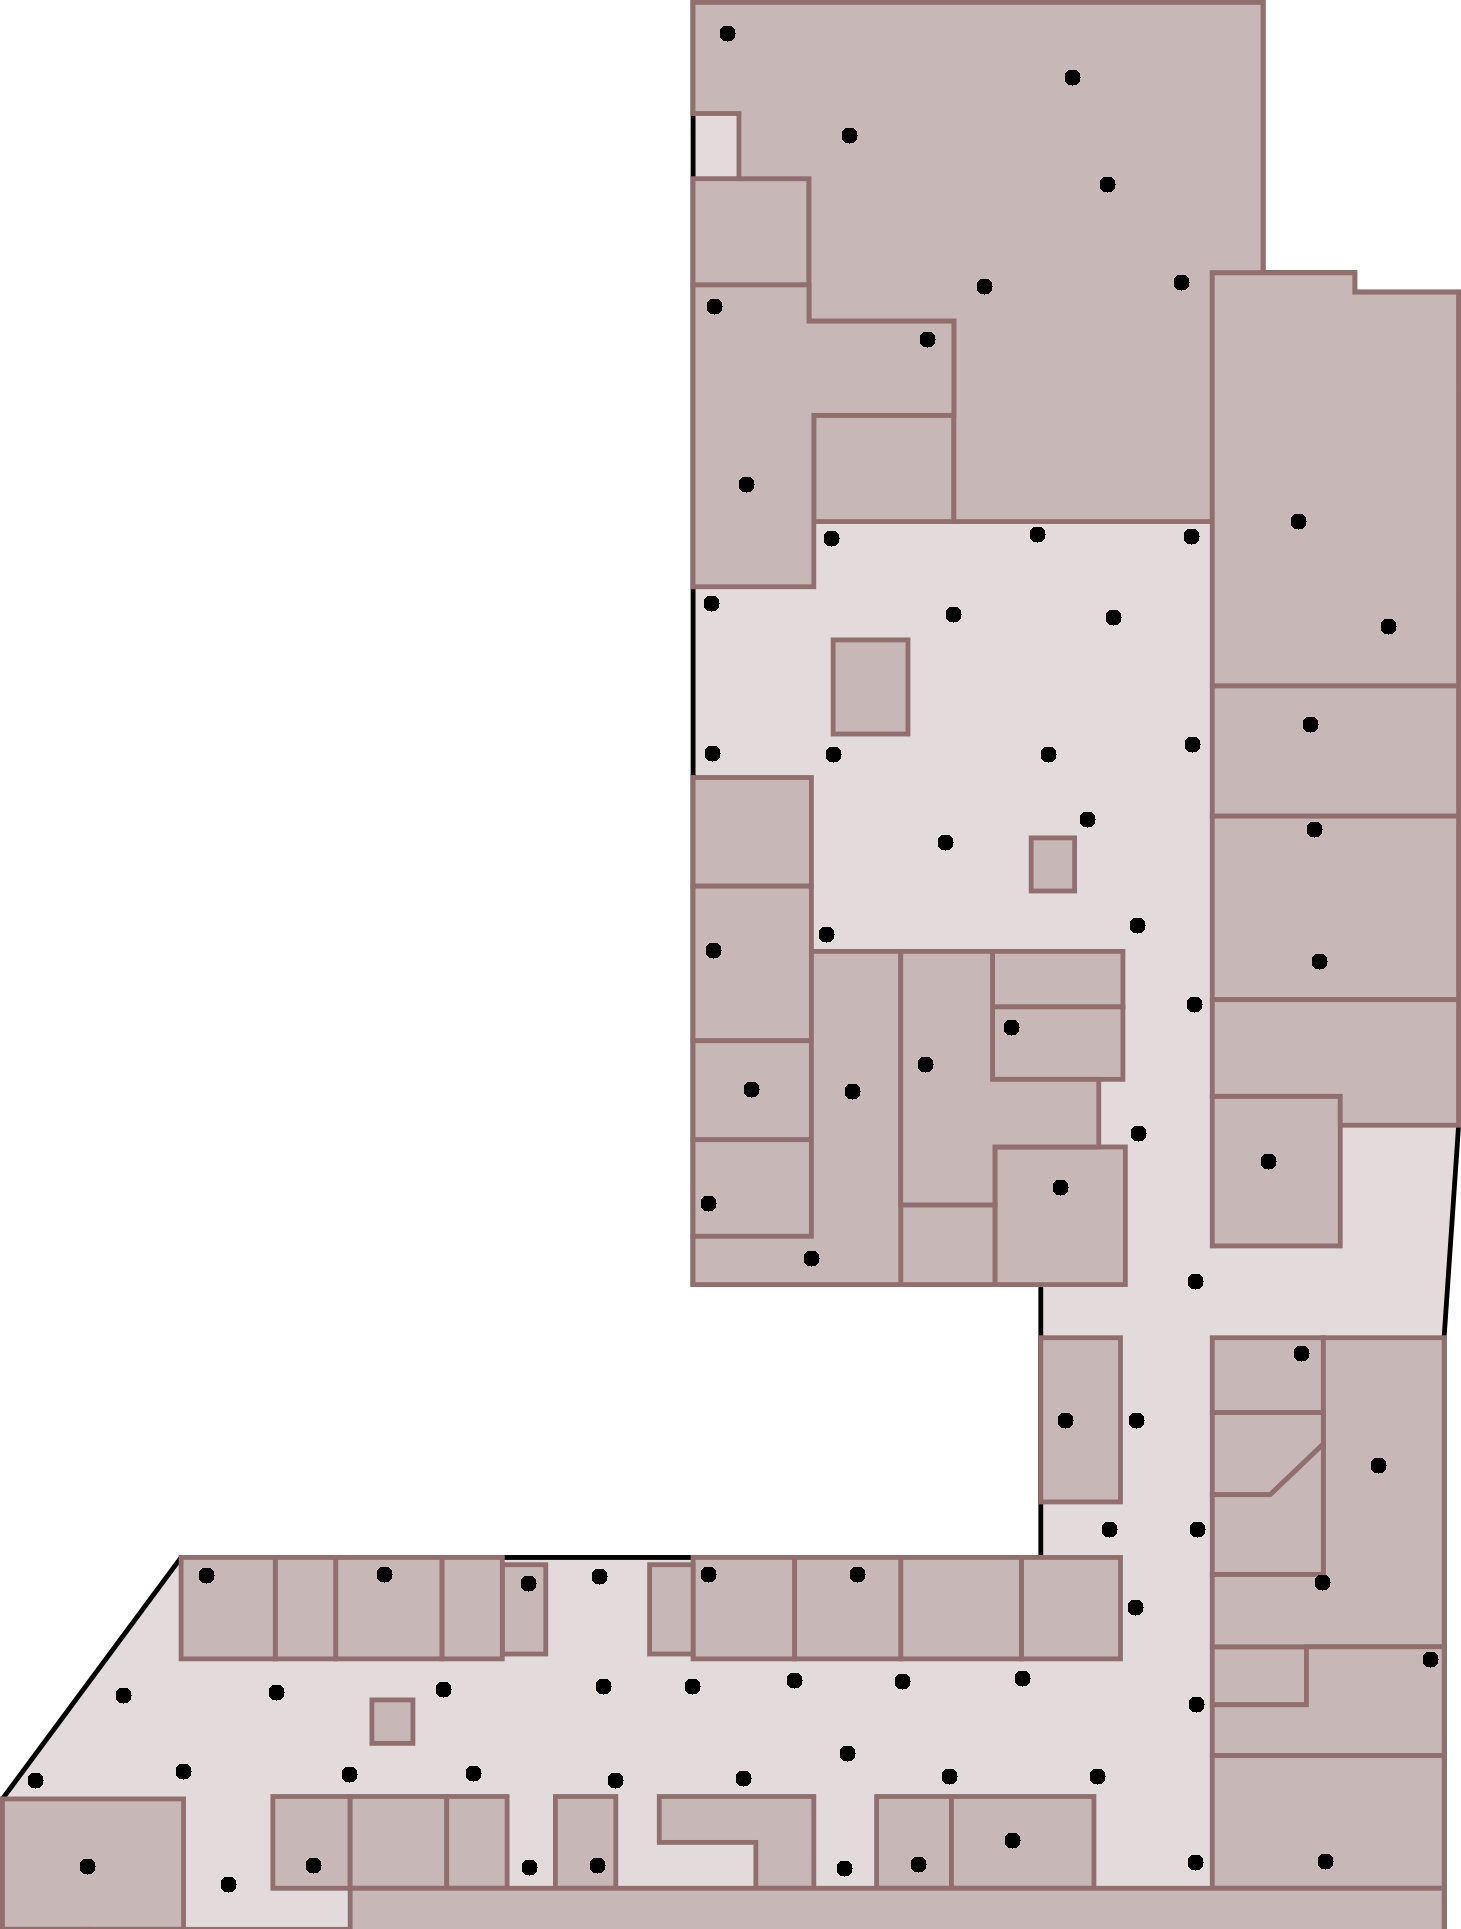
\includegraphics[width=7cm]{imatges/planol_log.png}
\caption{Punts on s'ha dut a terme la presa de dades per construir el mapa de ràdio.}
\label{fig:planol_log}
\end{center}
\end{figure}


Tenint en compte que el mapa de ràdio ha d'enregistrar els valors de les intensitats del senyal amb la màxima precisió possible, i que la presència d'usuaris en la potència de senyal rebut, es va considerar que la presa de dades per construir el mapa de ràdio s'havia de dur a terme en els moments de menys presència en el centre. El procés de presa de mesures per construir el mapa de ràdio va tenir lloc durant dos dies únicament entre les 8 i les 9 del matí. Dins les botigues, eñ procés es va dur a terme des del moment d'obertura dels locals comercials i només fins que l'absència de clients permetés una presa de dades convenient (normalment entre 30 i 60 minuts).El nombre de mesures dins botigues varia segons l'àrea ocupada per cada una.

Com que que a l'AirPlace Logger es poden definir la quantitat de mostres a prendre en cada punt a localitzar i l'interval de temps entre mostres, també s'ha de tenir en compte quins valors fixar. Com que el senyal rebut des d'un punt d'accés WiFi fluctua notablement i la potència rebuda mesurada varia al llarg del temps que dur la presa de les mostres, s'ha cregut convenient enregistrar el màxim nombre de mostres possibles, en aquest cas 30. D'aquesta manera s'assegura una millor mostra estadística a la hora de calcular la potència mitjana. L'interval entre cada mostra s'ha fixat en 1 segon, ja que mig segon entre mostres podria resultar en una mostra poc fluctuant, i dos segons hauria allargat massa el temps de presa de dades. A la figura \ref{fig:fluctuacio} es mostra la variació de la potència del senyal rebut en un punt al llarg de les 30 mostres. Com s'observa, en un punt la intensitat rebuda pot variar fins a 15 dbm, el que influeix en la poca precisió dels sistemes de localització per WiFi.

\begin{figure}[ht]
\begin{center}
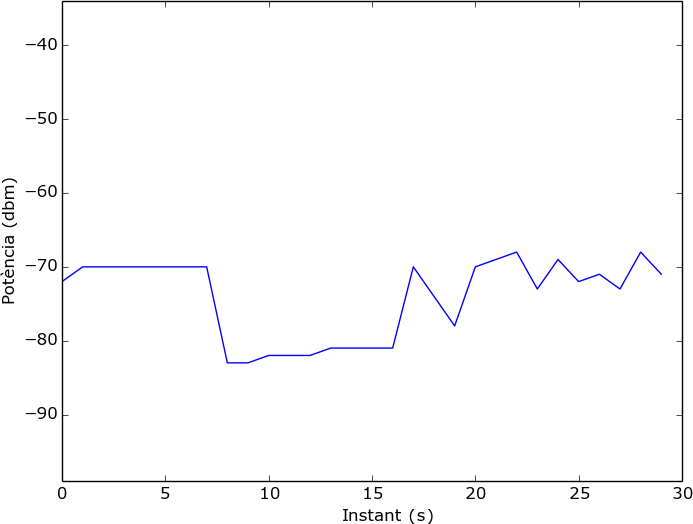
\includegraphics[width=7cm]{imatges/fluctuacio.png}
\caption{Variació de la potència del senyal rebut per la MAC f8:63:94:9c:2e:db al punt P74.}
\label{fig:fluctuacio}
\end{center}
\end{figure}
